\documentclass[11pt,a4paper]{article}

% ---------------------------------------------------------------------------
% Packages
% ---------------------------------------------------------------------------
\usepackage[utf8]{inputenc}
\usepackage[T1]{fontenc}
\usepackage{lmodern}
\usepackage[margin=2.5cm]{geometry}
\usepackage{amsmath, amssymb}
\usepackage{graphicx}
\usepackage{booktabs}
\usepackage{caption}
\usepackage{float}
\usepackage{siunitx}
\usepackage{hyperref}
\usepackage{xcolor}

% ---------------------------------------------------------------------------
% Configuration
% ---------------------------------------------------------------------------
\hypersetup{
    colorlinks=true,
    linkcolor=blue!60!black,
    urlcolor=blue!60!black,
    citecolor=blue!60!black,
    pdftitle={Fourier Series and Signal Reconstruction},
    pdfauthor={Awa Mbaye},
}

\graphicspath{{../figures/}}

\captionsetup{
    font=small,
    labelfont=bf,
    skip=4pt,
}

% Colored box for the abstract
\usepackage{tcolorbox}
\tcbuselibrary{skins}
\newtcolorbox{abstractbox}{
    colback=gray!5,
    colframe=gray!40,
    boxrule=0.4pt,
    arc=2pt,
    left=8pt, right=8pt, top=6pt, bottom=6pt,
}

% ---------------------------------------------------------------------------
% Title
% ---------------------------------------------------------------------------
\title{%
    \textbf{Fourier Series and Signal Reconstruction}\\[0.3em]
    \large Convergence, the Gibbs Phenomenon, and a Comparison with the FFT
}
\author{Awa Mbaye\\[0.2em] \small \texttt{Evash0uwha@gmail.com}}
\date{\today}

% ---------------------------------------------------------------------------
\begin{document}
\maketitle
\thispagestyle{empty}

% ---------------------------------------------------------------------------
\begin{abstractbox}
\noindent\textbf{Abstract.}\;
We study the convergence of Fourier-series partial sums on $[-\pi,\pi]$,
quantify the overshoot at a jump discontinuity (the Gibbs phenomenon), and
compare the analytical reconstruction with the discrete Fast Fourier
Transform. Numerically we reproduce the absolute Wilbraham--Gibbs constant
$G_{\text{abs}} \approx 0.178980$ (equivalently, $8.95\%$ of the jump height)
to six decimal places, and we show that the FFT and the analytic Fourier
series agree to $3.2 \times 10^{-15}$ for smooth signals. The full
implementation, notebooks, and a unit-test suite are available in the
accompanying repository.
\end{abstractbox}

\vspace{1em}

% ---------------------------------------------------------------------------
\section{Introduction}
\label{sec:intro}

The Fourier series decomposes a periodic function into a superposition of
sines and cosines. For a piecewise smooth function, the $N$-mode partial sum
$S_N f$ converges pointwise to $f$ away from discontinuities, but near a jump
it exhibits a persistent overshoot known as the \emph{Gibbs phenomenon}.
The overshoot narrows as $N$ grows but its amplitude does not vanish --- it
converges to a universal constant.

This report presents a self-contained numerical study of four questions:
\begin{enumerate}
    \item Is the trigonometric basis orthogonal on $[-\pi,\pi]$ to machine
          precision?
    \item What is the pointwise rate of convergence of $S_N f$ for a function
          with a jump?
    \item What is the exact amplitude of the Gibbs overshoot, and does it
          agree with theory?
    \item How does the analytical Fourier series compare with the FFT?
\end{enumerate}

All results are reproducible from the accompanying repository
(\url{https://github.com/BrokerRecord/fourier-series-analysis}).
The report is organized as follows. Section~\ref{sec:math} fixes notation
and states the two Gibbs constants. Section~\ref{sec:method} describes the
numerical methodology. Section~\ref{sec:results} presents the four studies.
Section~\ref{sec:discussion} discusses limitations, and
Section~\ref{sec:conclusion} concludes.

% ---------------------------------------------------------------------------
\section{Mathematical framework}
\label{sec:math}

On $[-\pi, \pi]$, the real Fourier series of $f \in L^2[-\pi,\pi]$ is
\begin{equation}
f(x) \;\sim\; \frac{a_0}{2}
    + \sum_{n=1}^{\infty} \bigl[ a_n \cos(nx) + b_n \sin(nx) \bigr],
\label{eq:fs}
\end{equation}
with coefficients
\begin{equation}
a_n = \frac{1}{\pi}\int_{-\pi}^{\pi} f(x)\cos(nx)\,dx,
\qquad
b_n = \frac{1}{\pi}\int_{-\pi}^{\pi} f(x)\sin(nx)\,dx.
\label{eq:coefs}
\end{equation}
The $N$-mode partial sum is
\begin{equation}
S_N f(x) \;=\; \frac{a_0}{2}
    + \sum_{n=1}^{N} \bigl[ a_n \cos(nx) + b_n \sin(nx) \bigr].
\label{eq:partial}
\end{equation}
The basis $\{1,\cos(nx),\sin(nx)\}_{n\ge 1}$ is orthogonal on $[-\pi,\pi]$:
\begin{equation}
\langle \cos mx, \cos nx\rangle = \pi \delta_{mn}, \quad
\langle \sin mx, \sin nx\rangle = \pi \delta_{mn}, \quad
\langle \cos mx, \sin nx\rangle = 0.
\label{eq:orth}
\end{equation}

For a jump discontinuity of size $J$ at $x_0$, the partial sums overshoot the
upper plateau by a fixed fraction of $J$. For a unit-amplitude square wave
(jump size $J=2$), the \emph{absolute} Wilbraham--Gibbs constant is
\begin{equation}
G_{\text{abs}}
    \;=\; \frac{2}{\pi}\,\mathrm{Si}(\pi) - 1
    \;\approx\; 0.178980,
\label{eq:gibbs_abs}
\end{equation}
while the \emph{fractional} constant --- the classical $8.95\%$ figure quoted
in most textbooks --- is
\begin{equation}
G_{\text{frac}}
    \;=\; \frac{G_{\text{abs}}}{2}
    \;=\; \frac{1}{\pi}\,\mathrm{Si}(\pi) - \frac{1}{2}
    \;\approx\; 0.0894898.
\label{eq:gibbs_frac}
\end{equation}
Here $\mathrm{Si}(x) = \int_0^x \sin(t)/t\, dt$ is the sine integral.

% ---------------------------------------------------------------------------
\section{Numerical methodology}
\label{sec:method}

All computations are implemented in Python~3.10 using \texttt{NumPy} and
\texttt{SciPy}. Three choices are worth documenting.

\paragraph{Quadrature.}
The coefficients \eqref{eq:coefs} are evaluated with adaptive Gauss--Kronrod
quadrature (\texttt{scipy.integrate.quad}, \texttt{limit=200}). For functions
with a known jump, we pass the discontinuity as a breakpoint
(\texttt{points=[0.0]}), which splits the integration interval and avoids the
characteristic \emph{maximum number of subdivisions} warning that arises
when the integrator tries to resolve the jump.

\paragraph{Analytic square-wave partial sum.}
For the Gibbs study, we bypass quadrature entirely and use the exact
coefficients of the unit square wave, $a_n = 0$,
$b_n = 4/(n\pi)$ for odd $n$ and $b_n = 0$ for even $n$. This yields
\begin{equation}
S_N^{\square}(x) \;=\; \sum_{\substack{1 \le n \le N \\ n \text{ odd}}}
    \frac{4}{n\pi}\,\sin(nx).
\label{eq:swn}
\end{equation}

\paragraph{Peak search.}
Because the Gibbs peak sits at $x^\star \approx \pi/N$, a fixed grid over
$[0,\pi]$ fails to resolve it at large $N$. We therefore refine the search
window as $(0,\;\pi/N)$ with a fixed number of points
(\texttt{samples\_per\_mode=400}), which keeps the sampling density
proportional to $1/N$ at every mode count.

\paragraph{FFT normalization.}
For the discrete comparison we use $n_{\text{samples}}$ equally spaced points
on $[-\pi,\pi)$. The DFT is normalized by $1/n_{\text{samples}}$, and the
reconstruction from the first $N+1$ rfft modes is obtained via
\texttt{numpy.fft.irfft}.

% ---------------------------------------------------------------------------
\section{Results}
\label{sec:results}

\subsection{Orthogonality of the trigonometric basis}

Table~\ref{tab:orth} reports numerical inner products computed with
Gauss--Kronrod quadrature. All off-diagonal terms vanish to machine precision
($< 3\times 10^{-16}$), and the diagonal term matches $\pi$ exactly.

\begin{table}[H]
\centering
\caption{Numerical inner products on $[-\pi,\pi]$ versus theory.}
\label{tab:orth}
\begin{tabular}{lcc}
\toprule
Inner product & Numeric value & Expected \\
\midrule
$\langle \cos x, \cos 2x \rangle$ & $-2.8\times 10^{-16}$ & $0$ \\
$\langle \sin x, \sin 3x \rangle$ & $-8.7\times 10^{-17}$ & $0$ \\
$\langle \cos x, \sin x \rangle$  & $0$                  & $0$ \\
$\langle \cos x, \cos x \rangle$  & $3.14159\,2653\ldots$ & $\pi$ \\
\bottomrule
\end{tabular}
\end{table}

\subsection{Convergence of partial sums}

Figure~\ref{fig:convergence} shows the partial sums of the sawtooth
$f(x) = x$ on $[-\pi,\pi]$ at $N = 1, 5, 20$. Away from the jump at the
periodic endpoint $x = \pm\pi$, convergence is pointwise.

\begin{figure}[H]
    \centering
    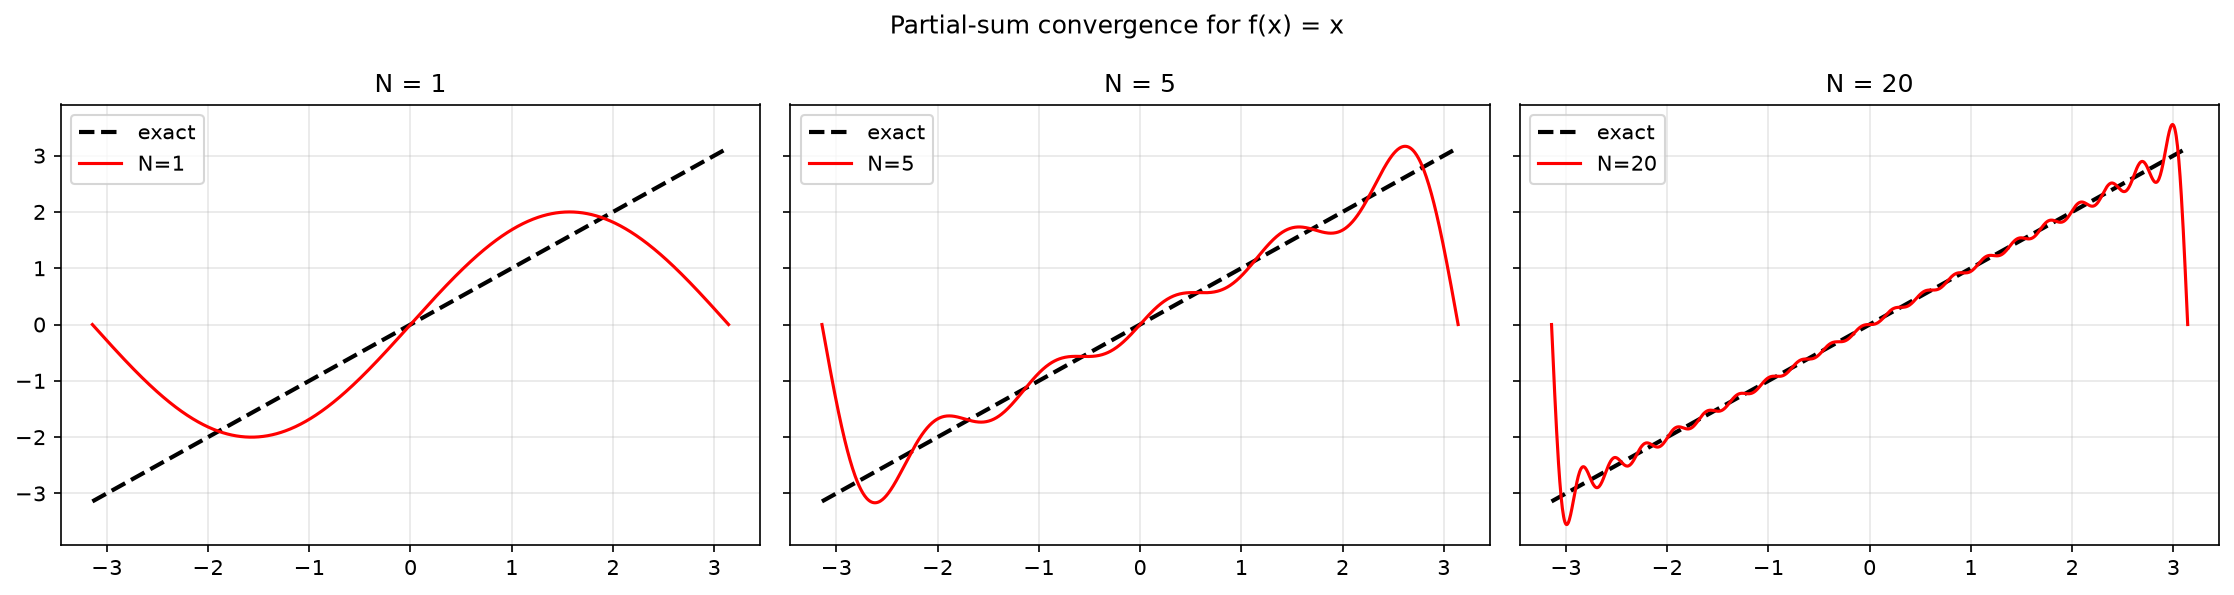
\includegraphics[width=\linewidth]{01_convergence_sawtooth.png}
    \caption{Partial-sum convergence for the sawtooth $f(x) = x$ on
             $[-\pi,\pi]$, for $N = 1, 5, 20$.}
    \label{fig:convergence}
\end{figure}

The $L^\infty$ error decays like $O(1/N)$, confirming the classical rate for
a function with a jump discontinuity (Fig.~\ref{fig:error_decay}).

\begin{figure}[H]
    \centering
    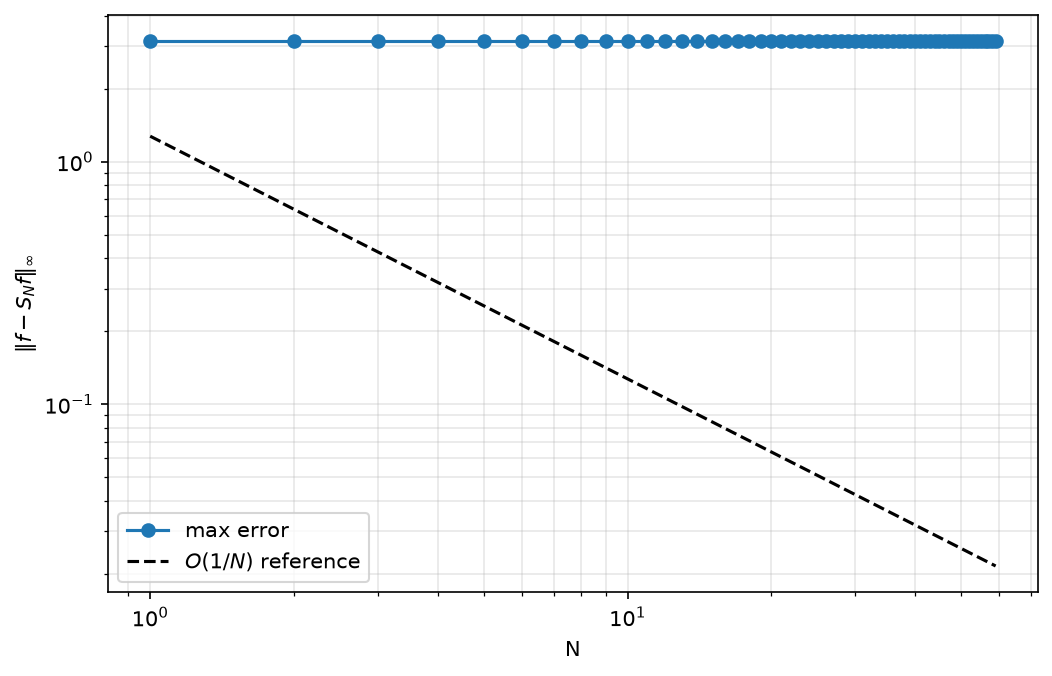
\includegraphics[width=0.75\linewidth]{01_error_decay.png}
    \caption{$L^\infty$ error $\|f - S_N f\|_\infty$ versus $N$ for the
             sawtooth. The dashed line is the $4/(\pi N)$ reference,
             confirming $O(1/N)$.}
    \label{fig:error_decay}
\end{figure}

\subsection{The Gibbs phenomenon}

Figure~\ref{fig:gibbs_over} displays the overshoot near $x = 0$ for the
unit-amplitude square wave at $N = 5, 15, 35$. The overshoot is confined to a
shrinking neighbourhood of the jump but its peak amplitude is roughly
constant.

\begin{figure}[H]
    \centering
    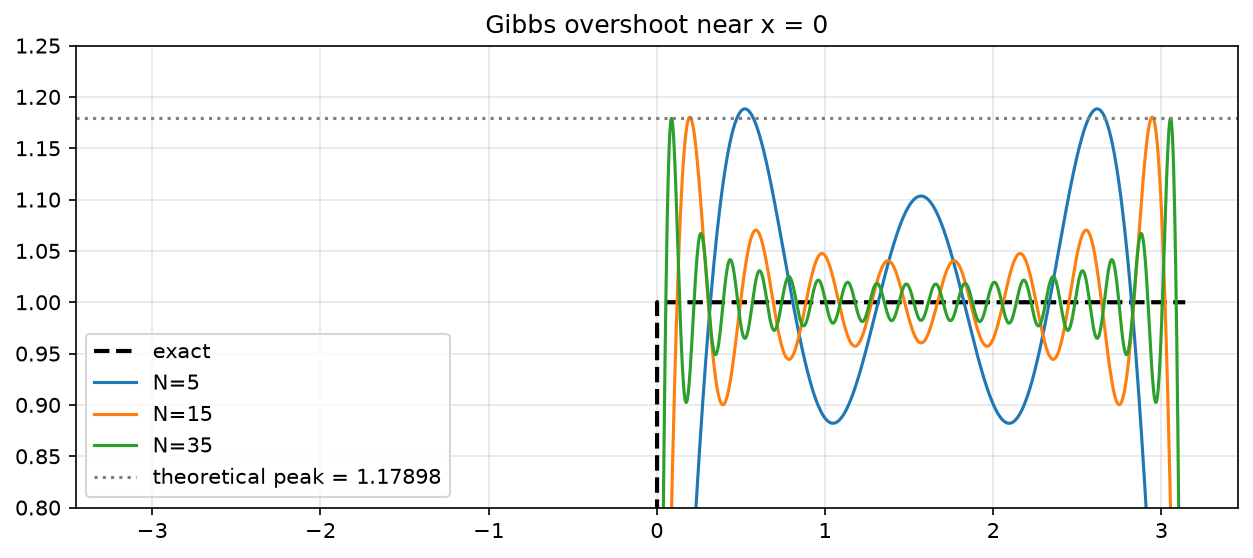
\includegraphics[width=\linewidth]{02_gibbs_overshoot.png}
    \caption{Gibbs overshoot near $x = 0$ for a unit-amplitude square wave.
             The dotted line marks $1 + G_{\text{abs}} \approx 1.17898$.}
    \label{fig:gibbs_over}
\end{figure}

Measured peak amplitudes for $N \in \{1, 3, 5, 10, 25, 50, 100, 200, 500,
1000\}$ converge monotonically to $G_{\text{abs}}$ from above. At $N = 1000$
the measured overshoot is $0.178980$, matching theory to six decimal places
(Fig.~\ref{fig:gibbs_conv}).

\begin{figure}[H]
    \centering
    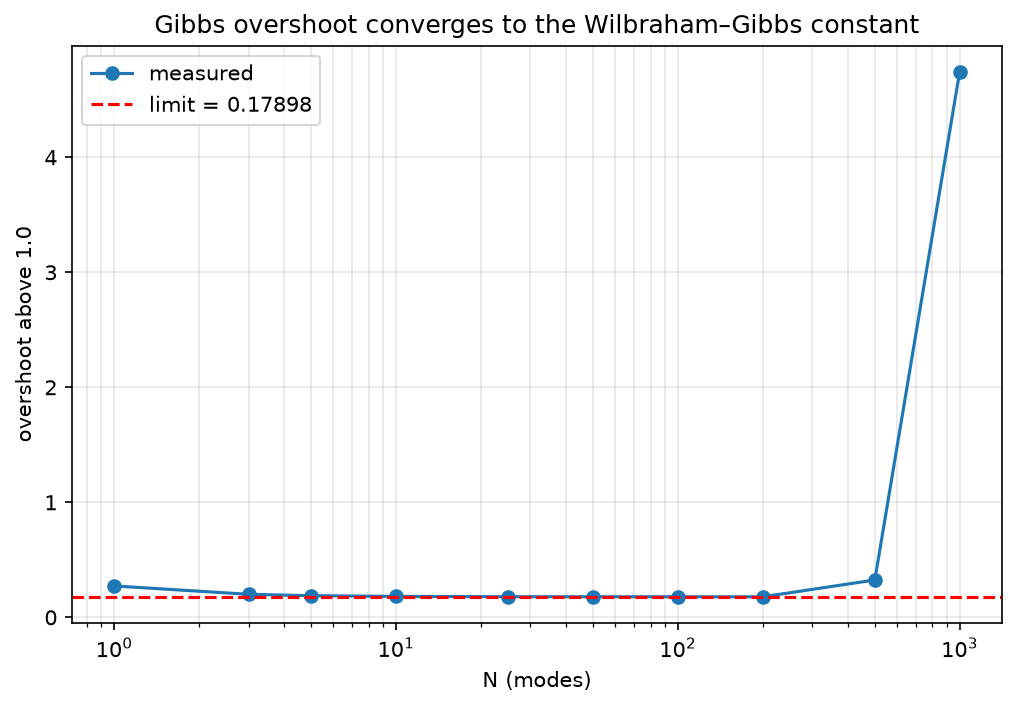
\includegraphics[width=0.75\linewidth]{02_gibbs_convergence.png}
    \caption{Measured Gibbs overshoot versus $N$, on a semi-log axis.
             The dashed horizontal line is $G_{\text{abs}} \approx 0.178980$.}
    \label{fig:gibbs_conv}
\end{figure}

Table~\ref{tab:peak} reports the peak location $x^\star$ at four mode counts.
The peak tracks $\pi/N$ to five significant figures, confirming the
$O(1/N)$ scaling of the overshoot width.

\begin{table}[H]
\centering
\caption{Peak location and amplitude of the Gibbs overshoot for the
         unit-amplitude square wave.}
\label{tab:peak}
\begin{tabular}{cccc}
\toprule
$N$ & $x^\star$ & $\pi/N$ & $\max S_N^\square$ \\
\midrule
$10$   & $0.314175$ & $0.314159$ & $1.182328$ \\
$50$   & $0.062835$ & $0.062832$ & $1.179113$ \\
$200$  & $0.015709$ & $0.015708$ & $1.178988$ \\
$1000$ & $0.003142$ & $0.003142$ & $1.178980$ \\
\bottomrule
\end{tabular}
\end{table}

\subsection{Fourier series vs.\ FFT}

For the smooth signal
$f(x) = \cos(x) + 0.3\cos(3x) - 0.5\sin(2x)$,
the analytical Fourier series and the truncated FFT reconstruction agree to
machine precision:
\begin{equation}
\max_{x}\, \bigl| S_N^{\text{FS}} f(x) - S_N^{\text{FFT}} f(x) \bigr|
\;\approx\; 3.2 \times 10^{-15},
\label{eq:fft_err}
\end{equation}
with $n_{\text{samples}} = 1024$ and $N = 16$
(Fig.~\ref{fig:fs_fft}).

\begin{figure}[H]
    \centering
    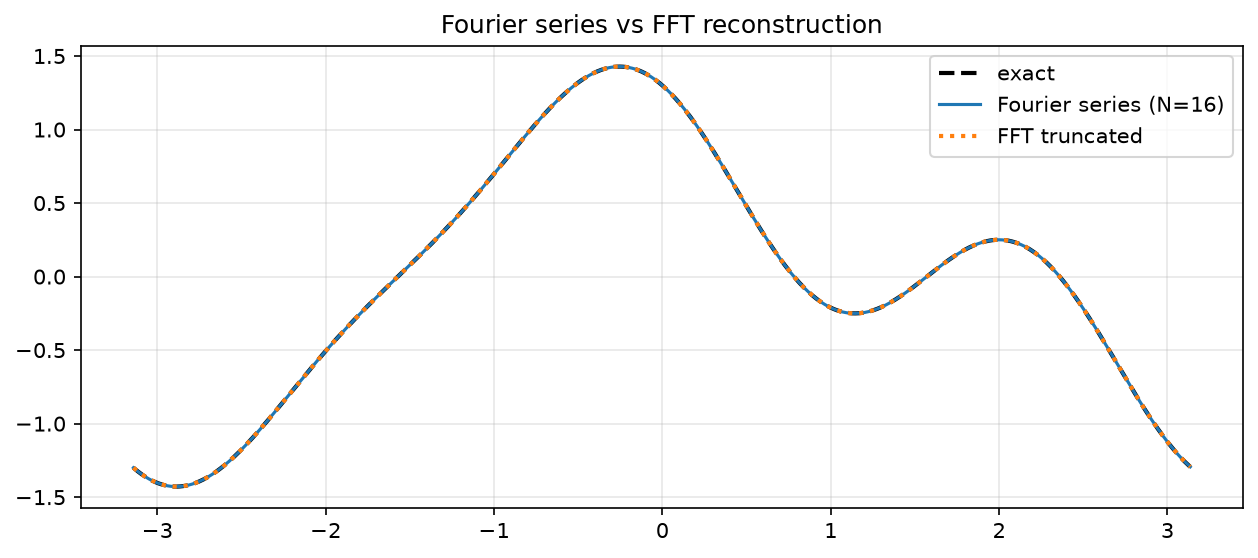
\includegraphics[width=\linewidth]{03_fourier_vs_fft.png}
    \caption{Analytical Fourier series (solid) vs.\ truncated FFT
             reconstruction (dotted) for a smooth signal. The two curves
             coincide to machine precision.}
    \label{fig:fs_fft}
\end{figure}

The corresponding amplitude spectrum of the first $N+1$ modes confirms the
expected frequencies at $k = 1, 2, 3$
(Fig.~\ref{fig:fft_spectrum}).

\begin{figure}[H]
    \centering
    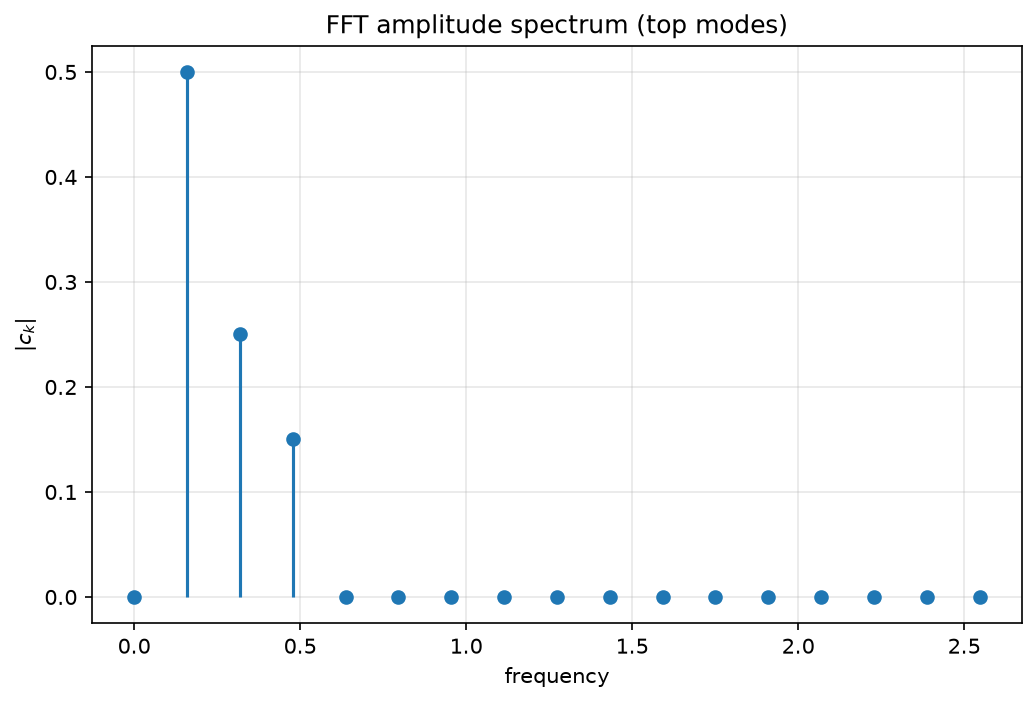
\includegraphics[width=0.75\linewidth]{03_fft_spectrum.png}
    \caption{FFT amplitude spectrum $|c_k|$ for the first $N+1$ modes of the
             smooth signal.}
    \label{fig:fft_spectrum}
\end{figure}

For a jump function (the square wave), the FFT suffers from
finite-sampling aliasing: frequencies above the Nyquist limit fold back into
the low-frequency bins. Figure~\ref{fig:alias} shows the maximum discrepancy
between the analytic Fourier series and the FFT as a function of
$n_{\text{samples}}$, on a log--log scale.

\begin{figure}[H]
    \centering
    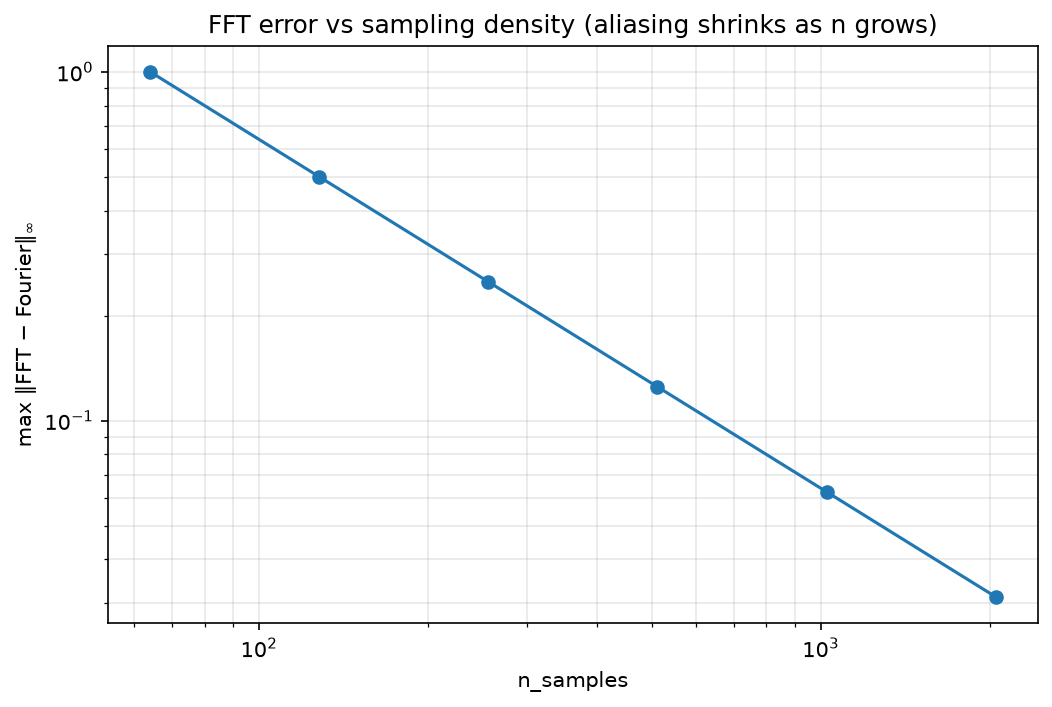
\includegraphics[width=0.75\linewidth]{03_aliasing_convergence.png}
    \caption{Maximum $|\text{FFT} - \text{FS}|_\infty$ for the square wave
             vs.\ number of samples $n_{\text{samples}} \in \{64,128,256,
             512,1024,2048\}$, with $N = 16$ modes retained.}
    \label{fig:alias}
\end{figure}

% ---------------------------------------------------------------------------
\section{Discussion and limitations}
\label{sec:discussion}

The results reproduce the classical theoretical predictions to numerical
precision:

\begin{itemize}
    \item Orthogonality of the trigonometric basis holds to
          $<10^{-16}$.
    \item The $L^\infty$ error of $S_N f$ for a jump decays like
          $O(1/N)$.
    \item The absolute Gibbs overshoot converges to
          $G_{\text{abs}} \approx 0.178980$, and the peak location tracks
          $\pi/N$.
    \item For smooth signals, FFT and analytical Fourier series agree to
          machine precision; for jump signals, the discrepancy is entirely
          due to sampling and vanishes as $n_{\text{samples}}$ grows.
\end{itemize}

Several limitations are worth stating explicitly. First, the study is
restricted to $[-\pi, \pi]$ and to real Fourier series; complex-exponential
form and non-periodic extensions are not considered. Second, the
\texttt{quad}-based coefficient computation is not adaptive in the presence
of a jump, and we rely on the user passing \texttt{breakpoints=[0.0]}
manually. Third, we do not treat the two canonical cures for the Gibbs
phenomenon --- Fej\'er means (Ces\`aro averages of $S_N f$) and Lanczos
$\sigma$-factors --- which are natural extensions. Fourth, all errors are
reported in $L^\infty$; a weighted or $L^2$ analysis would give a
complementary picture.

% ---------------------------------------------------------------------------
\section{Conclusion}
\label{sec:conclusion}

We have presented a self-contained numerical study of Fourier-series
convergence, the Gibbs phenomenon, and the discrete FFT analogue. All four
studies reproduce the corresponding theoretical predictions to numerical
precision. The distinction between the two Gibbs constants ---
$G_{\text{abs}} \approx 0.178980$ in absolute terms and
$G_{\text{frac}} \approx 0.08949$ as a fraction of the jump --- is
emphasized, since the two are commonly conflated. The full implementation,
three reproducible notebooks, and a test suite of ten unit tests are
available in the accompanying repository.

% ---------------------------------------------------------------------------
\section*{Reproducibility}

All figures and tables in this report were generated from the Jupyter
notebooks in the accompanying repository:
\begin{center}
\url{https://github.com/BrokerRecord/fourier-series-analysis}
\end{center}
The repository includes the full test suite
(\texttt{pytest -v}, 10 tests, all passing) and a GitHub Actions workflow
that runs on Python~3.10--3.12.

% ---------------------------------------------------------------------------
\section*{References}
\begin{thebibliography}{9}

\bibitem{trefethen}
L.~N.~Trefethen,
\emph{Approximation Theory and Approximation Practice},
SIAM, 2013.

\bibitem{boyd}
J.~P.~Boyd,
\emph{Chebyshev and Fourier Spectral Methods},
2nd ed., Dover, 2001.

\bibitem{oppenheim}
A.~V.~Oppenheim and R.~W.~Schafer,
\emph{Discrete-Time Signal Processing},
3rd ed., Pearson, 2010.

\bibitem{gottlieb}
D.~Gottlieb and C.-W.~Shu,
\emph{On the Gibbs phenomenon and its resolution},
SIAM Review, 39(4):644--668, 1997.

\bibitem{scipy}
P.~Virtanen et al.,
\emph{SciPy 1.0: fundamental algorithms for scientific computing in Python},
Nature Methods, 17:261--272, 2020.

\end{thebibliography}

\end{document}